
\begin{flushleft}
	
	\begin{itemize}
		\item Unicode is the universal character encoding.
		\item The Unicode Standard provides a unique number for every character, no matter what platform, device, application or language. 
		
		\begin{tcolorbox}[breakable,notitle,boxrule=-0pt,colback=code,colframe=code]
			\color{white}
			\fontdimen2\font=8pt
			var='$\backslash$u0950 $\backslash$u0918$\backslash$u0968 $\backslash$u0975 $\backslash$u0937$\backslash$u0926' \newline
			print(var)
			\fontdimen2\font=4pt
		\end{tcolorbox}
		
		Output:
		\begin{figure}[h!]
			\centering
			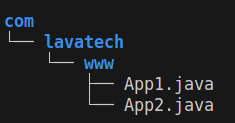
\includegraphics[scale=0.8]{content/chapter2/images/new.png}
		\end{figure}
		
		
	\end{itemize}
		


		
\end{flushleft}

\newpage

